\section{Absolutely Continuous Random Variables}
    We begin by reviewing the definition of an absolutely continuous random variable. Let $X$ be a random variable defined on a probability space $(\Omega, \mathcal{A}, P)$ and taking values in $\mathbb{R}$. A random variable $X$ is called \textit{absolutely continuous} if there exists a function $f_X: \mathbb{R} \to \mathbb{R}^+$, called the \textit{density} of $X$, such that the cumulative distribution function (CDF) $F_X$ of $X$ can be written as:
    \[
    F_X(x) = P(X \leq x) = \int_{-\infty}^{x} f_X(t) \, dt \quad \text{for all } x \in \mathbb{R}.
    \]
    Thus, the random variable is absolutely continuous if its distribution function can be expressed as the integral of a non-negative function, $f_X$, called the density.
    
    \paragraph{Properties of the Density Function}
    The density function $f_X$ must satisfy the following two properties:
    \begin{enumerate}
        \item The integral of $f_X$ over the entire real line must equal 1:
        \[
        \int_{-\infty}^{\infty} f_X(x) \, dx = 1.
        \]
        This ensures that the total probability over the real line is 1, as required by the probability measure since
        \[
        1 = P(X \in \mathcal\mathbb{R}) = \int_{-\infty}^{\infty} f_X(x) \, dx 
        \].
        \item For any interval $[a, b]$, the probability that $X$ lies within this interval is given by:
        \[
        P(X\in (a,b)) = F_X(b) - F_X(a) = P(a \leq X \leq b) = \int_{a}^{b} f_X(x) \, dx.
        \]
    \end{enumerate}
    
    \paragraph{Relation Between Distribution Function and Density}
    The cumulative distribution function (CDF) $F_X(x)$ represents the probability that $X$ takes a value less than or equal to $x$. The difference $F_X(b) - F_X(a)$ represents the probability that $X$ falls within the interval $[a, b]$:
    \[
    P(a \leq X \leq b) = F_X(b) - F_X(a).
    \]
    By the fundamental theorem of calculus, this difference can also be expressed as the integral of the density function:
    \[
    P(a \leq X \leq b) = \int_{a}^{b} f_X(x) \, dx.
    \]
    
    \paragraph{Interpretation of Density and Probability}
    The value of $f_X(x)$ at a particular point $x$ does not determine the probability that $X = x$. In fact, for an absolutely continuous random variable, the probability that $X$ takes any specific value is 0:
    \[
    P(X = a) = \int_{a}^{a} f_X(x) \, dx = 0.
    \]
    The probability is instead distributed over intervals, not individual points. This contrasts with discrete random variables, where probabilities are concentrated on specific values. It is important to note that modifying the value of the density function at a single point does not affect the integral. This means that even if the density function has a discontinuity at $x = 0$, the integral remains the same. The distribution function, $F_X(x)$, is continuous, and the value of $f_X(x)$ at a single point does not impact the probability calculations. \newline
    In practice, we will often approximate continuous random variables using discrete random variables, especially when working with large data sets or simulations.
    
    \section{Singular Distributions}
    We now turn to the concept of singular distributions. These are distributions that are continuous, but their CDF cannot be written as the integral of a density function. A random variable $X$ is called \textit{continuous} if its distribution function $F_X(x)$ is a continuous function of $x$. However, not all continuous random variables are absolutely continuous.
    
    \subsection{Singular Distributions}
    A singular distribution is a continuous random variable whose distribution function $F_X(x)$ cannot be expressed as the integral of a density function. These distributions are characterized by the fact that their derivative (if it exists) is 0 almost everywhere with respect to the Lebesgue measure. A well-known example of a singular distribution is the Cantor distribution.
    
    \paragraph{Cantor Function Example}
    The Cantor function is a famous example of a singular distribution. It is constructed by repeatedly removing middle thirds from the interval $[0, 1]$ and flattening the function over those intervals. This leads to a function $F_C(x)$ that is continuous and increases from 0 to 1 but has a derivative of 0 almost everywhere. In other words, $F_C(x)$ is continuous, but its derivative is 0 at almost every point.
    
    \paragraph{Key Properties}
    \begin{itemize}
        \item The Cantor function is continuous, but almost nowhere differentiable.
        \item The function increases from 0 to 1, but the increase occurs in a set of length 0 (a set that is uncountable but has Lebesgue measure 0).
        \item The derivative of the Cantor function is 0 almost everywhere, but integrating this derivative would yield 0, even though the function itself increases from 0 to 1.
    \end{itemize}
    This example demonstrates that the relationship between differentiation and integration can break down for certain continuous functions, leading to the existence of singular distributions.
    
    \section{Exponential Random Variable}
    A random variable $X$ is called an exponential random variable with parameter $\lambda > 0$ if its probability density function (PDF) is given by:
    \[
    f_X(x) = \begin{cases} 
    0 & \text{if } x < 0, \\
    \lambda e^{-\lambda x} & \text{if } x \geq 0.
    \end{cases}
    \]
    Thus, for $x < 0$, the density is zero, and for $x \geq 0$, the density is $\lambda e^{-\lambda x}$.
    
    \paragraph{Behavior of the Density Function}
    At $x = 0$, the value of the density function is:
    \[
    f_X(0) = \lambda e^{-\lambda \cdot 0} = \lambda.
    \]
    \begin{figure}[h]
        \centering
        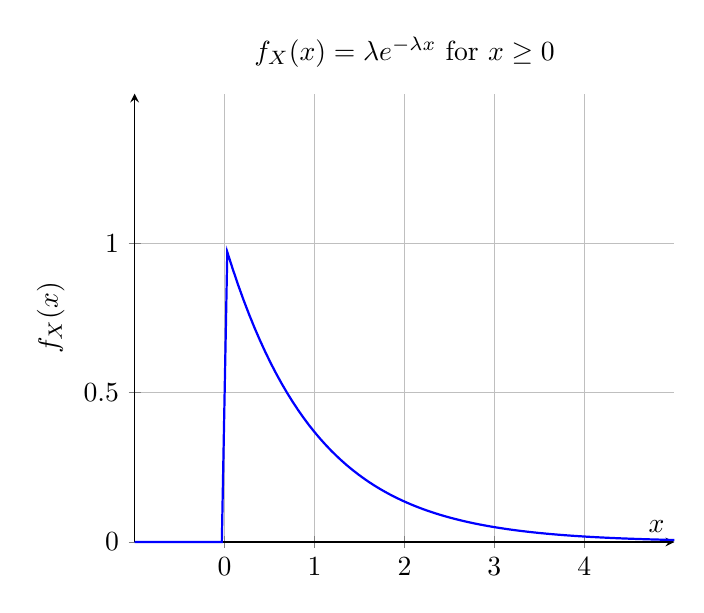
\begin{tikzpicture}
            \begin{axis}[
                title={$f_X(x) = \lambda e^{-\lambda x}$ for $x \geq 0$},
                xlabel={$x$},
                ylabel={$f_X(x)$},
                grid=major,
                domain=-1:5,
                samples=100,
                ymin=0, ymax=1.5,
                axis y line=left,
                axis x line=middle,
                xtick={0,1,2,3,4},
                ytick={0,0.5,1},
                enlargelimits=false,
                clip=false
            ]
            % Plot the function f_X(x)
            \addplot[color=blue, thick] 
            {(x < 0) * 0 + (x >= 0) * exp(-1 * x)}; % Assuming lambda = 1
            \end{axis}
        \end{tikzpicture}
        \caption{Plot of $f_X(x)$ with $\lambda = 1$}
    \end{figure}
    This means that the density starts at $\lambda$ when $x = 0$ and then decreases exponentially towards 0 as $x$ increases. The graph of this density function looks like a decaying exponential curve starting from $\lambda$ at $x = 0$ and approaching 0 as $x \to \infty$.
    
    \subsection{Cumulative Distribution Function (CDF)}
    The cumulative distribution function (CDF) $F_X(x)$ of the exponential random variable is the integral of the density function:
    \[
    F_X(x) = P(X \leq x) = \int_{-\infty}^{x} f_X(t) \, dt.
    \]
    To compute this, we must consider two cases depending on the value of $x$.
    
    \paragraph{Case 1: $x < 0$}
    For $x < 0$, the density function is zero, so the CDF is:
    \[
    F_X(x) = \int_{-\infty}^{x} 0 \, dt = 0.
    \]
    
    \paragraph{Case 2: $x \geq 0$}
    For $x \geq 0$, the CDF is computed as follows:
    \[
    F_X(x) = \int_0^{x} \lambda e^{-\lambda t} \, dt.
    \]
    The antiderivative of $\lambda e^{-\lambda t}$ is $-e^{-\lambda t}$, so we evaluate the integral:
    \[
    F_X(x) = \left[ -e^{-\lambda t} \right]_0^x = -e^{-\lambda x} + e^0 = 1 - e^{-\lambda x}.
    \]
    
    \paragraph{Summary of the CDF}
    Thus, the cumulative distribution function of the exponential random variable is:
    \[
    F_X(x) = \begin{cases} 
    0 & \text{if } x < 0, \\
    1 - e^{-\lambda x} & \text{if } x \geq 0.
    \end{cases}
    \]
    \section{Graph of the CDF}
    \begin{figure}[h]
        \centering
        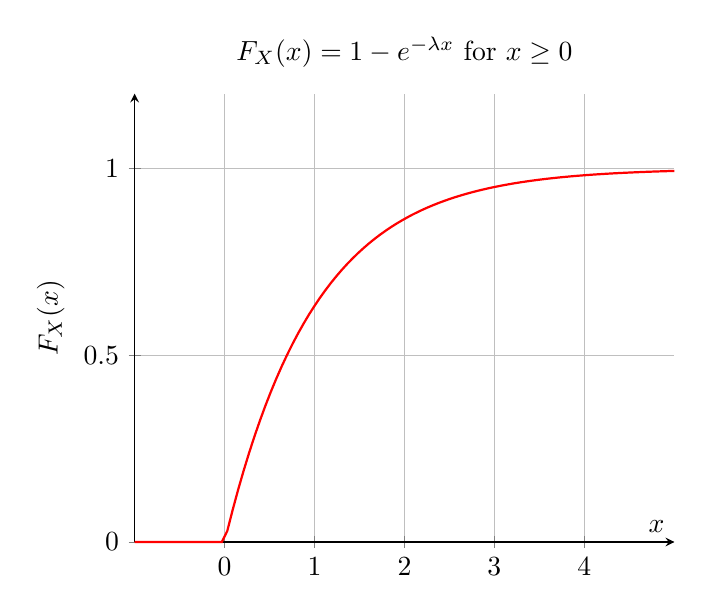
\begin{tikzpicture}
            \begin{axis}[
                title={$F_X(x) = 1 - e^{-\lambda x}$ for $x \geq 0$},
                xlabel={$x$},
                ylabel={$F_X(x)$},
                grid=major,
                domain=-1:5,
                samples=100,
                ymin=0, ymax=1.2,
                axis y line=left,
                axis x line=middle,
                xtick={0,1,2,3,4},
                ytick={0,0.5,1},
                enlargelimits=false,
                clip=false
            ]
            % Plot the function F_X(x)
            \addplot[color=red, thick] 
            {(x < 0) * 0 + (x >= 0) * (1 - exp(-1 * x))}; % Assuming lambda = 1
            \end{axis}
        \end{tikzpicture}
        \caption{Plot of $F_X(x)$ with $\lambda = 1$}
    \end{figure}
    The graph of the CDF is a continuous function that starts at 0 when $x < 0$ and increases smoothly towards 1 as $x \to \infty$. The CDF is a characteristic S-shaped curve that asymptotically approaches 1.
    
    \paragraph{Properties of the Exponential Distribution}
    The exponential distribution has several important properties:
    \begin{itemize}
        \item The density function is discontinuous at $x = 0$, but this does not affect the overall behavior of the distribution.
        \item The CDF is continuous everywhere, even though the density function has a jump at $x = 0$.
        \item The exponential distribution is an absolutely continuous distribution, meaning that it can be written as the integral of its density function.
    \end{itemize}

    \section{General Definition of Expectation}
    We now provide a more formal definition of the expectation for both discrete and continuous random variables. Although the method of computation differs depending on whether the random variable is discrete or continuous, the general concept of expectation remains the same.
    
    \paragraph{Discrete Random Variables}
    For a discrete random variable $X$ taking values $x_1, x_2, \dots$ with probabilities $P(X = x_i)$, the expectation is given by:
    \[
    \mathbb{E}[X] = \sum_{i} x_i P(X = x_i).
    \]
    
    \paragraph{Continuous Random Variables}
    For an absolutely continuous random variable $X$ with probability density function (PDF) $f_X(x)$, the expectation is given by:
    \[
    \mathbb{E}[X] = \int_{-\infty}^{\infty} x f_X(x) \, dx.
    \]
    In this case, the expectation is the integral of $x$ weighted by the density function $f_X(x)$.
    
    \section{Expectation of a Bernoulli Random Variable}
    Let $X$ be a Bernoulli random variable, denoted as $X \sim \text{Bernoulli}(p)$. This random variable takes the value 0 with probability $1 - p$, and the value 1 with probability $p$. The expectation (or mean) of $X$ is denoted by $\mathbb{E}[X]$.
    
    \paragraph{Definition of Expectation}
    The expectation of $X$ is defined as the weighted sum of its possible values, where the weights are given by the probabilities of each value. For the Bernoulli random variable:
    \[
    \mathbb{E}[X] = 0 \cdot P(X = 0) + 1 \cdot P(X = 1).
    \]
    Substituting the probabilities:
    \[
    \mathbb{E}[X] = 0 \cdot (1 - p) + 1 \cdot p = p.
    \]
    Thus, the expectation of a Bernoulli random variable with parameter $p$ is simply $p$.
    
    \subsection{General Case: Expectation of a Discrete Random Variable}
    Consider a more general discrete random variable $X$ that takes two possible values, $A$ and $B$, with probabilities $p$ and $1 - p$, respectively. The expectation is given by:
    \[
    \mathbb{E}[X] = A \cdot P(X = A) + B \cdot P(X = B).
    \]
    Substituting the probabilities:
    \[
    \mathbb{E}[X] = A \cdot p + B \cdot (1 - p).
    \]
    
    \section{Expectation of a Bernulli Random Variable}
    Let $X \sim \text{Bernulli}(n, p)$. The probability mass function of $X$ is given by:
    \[
    P(X = k) = \binom\mathbb{N}{k} p^k (1 - p)^{n - k} \quad \text{for } k = 0, 1, \dots, n.
    \]
    The expectation of $X$ is:
    \[
    \mathbb{E}[X] = \sum_{k=0}^\mathbb{N} k \cdot P(X = k) = \sum_{k=0}^\mathbb{N} k \cdot \binom\mathbb{N}{k} p^k (1 - p)^{n-k}.
    \]
    We can simplify this by observing that the term for $k = 0$ contributes nothing to the sum, so:
    \[
    \mathbb{E}[X] = \sum_{k=1}^\mathbb{N} k \cdot \binom\mathbb{N}{k} p^k (1 - p)^{n-k} \\
    \mathbb{E}[X] = \sum_{k=1}^\mathbb{N} k \cdot \frac{n!}{k!(n-k)!} p^k (1 - p)^{n-k}.
    \]
    Which becomes
    \[\sum_{k=1}^\mathbb{N}\frac{n!}{(k-1!)[(n-1)-(k-1)]!} p^k (1 - p)^{n-k} = \sum_{k=1}^\mathbb{N}n \cdot\frac{(n-1)!}{(k-1!)[(n-1)-(k-1)]!} p^k (1 - p)^{n-k} = \]
    \[
    = \sum_{k=1}^\mathbb{N}n\cdot \binom{n-1}{k-1} p^k (1 - p)^{n-k} = n\cdot p \cdot \sum_{k=1}^\mathbb{N} \binom{n-1}{k-1} p^{k-1} (1 - p)^{(n-1)-(k-1)}\]
    By using algebraic manipulation (binomial theorem and properties of factorials), it can be shown that:
    \[
    \mathbb{E}[X] = n \cdot p
    \]
    since the sum is equal to one given its definition (just substitute l = k-1).
    This is the expected number of successes in $n$ independent Bernoulli trials, each with probability $p$ of success.

        \section{Expectation of a Constant Random Variable}
    If $X$ is a constant random variable, i.e., $X = k$ with probability 1, then the expectation of $X$ is simply $k$:
    \[
    \mathbb{E}[X] = k.
    \]
    This is because $X$ only takes the value $k$ with probability 1, so the expectation is exactly $k$.
    
    \section{Geometric Random Variable}
    Consider a geometric random variable $X$ with parameter $p$, where $p \in (0, 1)$. The probability mass function of $X$ is given by:
    \[
    P(X = k) = (1 - p)^{k-1} p, \quad \text{for } k \in \mathbb{N}^+.
    \]
    The expectation of $X$ is:
    \[
    \mathbb{E}[X] = \sum_{k=1}^{\infty} k \cdot (1 - p)^{k-1} p.
    \]
    As an exercise, it can be proven that the expectation of a geometric random variable is:
    \[
    \mathbb{E}[X] = \frac{1}{p}.
    \]
    
    \section{General Case of Expectation for Discrete Random Variables}
    If $X$ is a discrete random variable taking countably infinite values, we define the expectation as:
    \[
    \mathbb{E}[X] = \sum_{x \in \mathbb{R}} x \cdot p_X(x),
    \]
    where $p_X(x) > 0$ for each value of $x$ in the support. This sum may be infinite or not well-defined, depending on the behavior of the probabilities and values of $X$.
    
    \subsection{Handling Infinite Sums}
    To handle infinite sums properly, we define:
    \[
    S^+ = \sum_{x \geq 0} x \cdot p_X(x) \quad \text{and} \quad S^- = \sum_{x < 0} (-x) \cdot p_X(x).
    \]
    These are the sums of the positive and negative parts of $X$. The expectation is well-defined if at least one of $S^+$ or $S^-$ is finite. If both $S^+$ and $S^-$ are finite, we say that $X$ is \textit{integrable} and the expectation is given by:
    \[
    \mathbb{E}[X] = S^+ - S^-.
    \]
    
    \subsection{Conditions for Well-Defined Expectation}
    The expectation is considered well-defined in the following cases:
    \begin{itemize}
        \item If $S^+ < \infty$ and $S^- = +\infty$, then $\mathbb{E}[X] = -\infty$.
        \item If $S^+ = +\infty$ and $S^- < \infty$, then $\mathbb{E}[X] = +\infty$.
        \item If $S^+ = S^- = \infty$, the expectation is undefined.
    \end{itemize}
    If both $S^+$ and $S^-$ are finite, then $X$ is integrable, and the expectation is finite.
    
    \section{$L^1$ and Integrable Random Variables}
    A key concept in probability is the space of \textit{integrable random variables}, denoted by $L^1(\Omega)$. We say that a random variable $X$ belongs to $L^1(\Omega)$ if and only if the expectation of the absolute value of $X$ is finite:
    \[
    \mathbb{E}[|X|] = \sum_{x \in \mathbb{R}} |x| P(X = x) < \infty.
    \]
    In simpler terms, a discrete random variable $X$ is integrable if the sum of the absolute values of $X$ multiplied by their corresponding probabilities converges.
    
    \paragraph{Definition of $L^1(\Omega)$}
    We define $L^1(\Omega)$ as the space of all integrable random variables on the probability space $\Omega$. Thus, a random variable $X \in L^1(\Omega)$ if and only if:
    \[
    \sum_{x \in \mathbb{R}} |x| P(X = x) < \infty.
    \]
    
    \subsection{Non-Negative Random Variables}
    In the special case of a discrete \textit{non-negative} random variable $Y$, the expectation is always well-defined. Since $Y \geq 0$, the negative part of $Y$ is zero, and we are guaranteed that the expectation of $Y$ will lie between 0 and $+\infty$:
    \[
    \mathbb{E}[Y] = \sum_{x \in \mathbb{R}^+} x P(Y = x).
    \]
    In the case of continuous random variables, the construction is similar, but we replace the summation with an integral.
    
    \subsection{Generalization of Expectation}
    We can generalize the definition of expectation to random variables that take an infinite number of values. If $X$ takes both positive and negative values, we divide the sum into two parts: 
    \[
    S^+ = \sum_{x \geq 0} x \cdot P(X = x), \quad S^- = \sum_{x < 0} (-x) \cdot P(X = x).
    \]
    The expectation is well-defined if at least one of $S^+$ or $S^-$ is finite. If both sums are finite, we say that $X$ is \textit{integrable}, and the expectation is:
    \[
    \mathbb{E}[X] = S^+ - S^-.
    \]
    If either $S^+$ or $S^-$ is infinite, the expectation may be $+\infty$, $-\infty$, or undefined (if both are infinite). The most interesting case is when both $S^+$ and $S^-$ are finite, making the expectation finite as well. In this case:
    \[
    \mathbb{E}[|X|] = S^+ + S^- < \infty.
    \]
    In this case we say that X is integrable, $X \in L^1(\Omega)$. \newline
    \textbf{Remark:} If $X$ is non-negative, $S^- = 0$, hence $\mathbb{E}[X]$ is always well-defined and lies in $[0, \infty]$.
    
    \paragraph{Expectation of a General Random Variable}
    To define the expectation for a general non-negative random variable $X$, we approximate $X$ from below using a sequence of non-negative discrete random variables $\{X_n\}$ such that:
    \[
    X_n(\omega) \leq X_{n+1}(\omega) \leq X(\omega), \quad \forall \omega.
    \]
    Then, we define:
    \[
    \mathbb{E}[X] = \lim_{n \to \infty} \mathbb{E}[X_n],
    \]
    where each $X_n$ is a discrete approximation of $X$. \newline
    The limit is independent of the specific sequence $\{X_n\}$, and thus $\mathbb{E}[X]$ is well-defined as either a finite number or $\infty$. \newline
    To approximate $X$ using $X_n$, for each $\omega$ and $n\geq 1, k\in \mathbb{N}$, we define:
    \[
    X_n(\omega) = \frac{k}{2^n}, \quad \text{where} \quad \frac{k}{2^n} \leq X(\omega) < \frac{k+1}{2^n}.
    \]
    This construction yields an increasing sequence of random variables, where each $X_n$ is discrete and takes values $0, \frac{1}{2^n}, \frac{2}{2^n}, \dots$, thereby forming an increasing sequence that converges to $X$.
    
    \paragraph{Expectation of a General Random Variable with Both Positive and Negative Values}
    For a general random variable $X:\Omega \rightarrow R$, we define:
    \[
    X^+ = \max(X, 0) \quad \text{and} \quad X^- = -\min(X, 0),
    \]
    note that they are both positive, so that:
    \[
    X = X^+ - X^- \quad \text{and} \quad |X| = X^+ + X^-.
    \]
    We say that $X$ admits an expectation if at least one of $\mathbb{E}[X^+]$ and $\mathbb{E}[X^-]$ is finite. \newline
    The most interesting case occurs when both $\mathbb{E}[X^+]$ and $\mathbb{E}[X^-]$ are finite. In this case, we define $X$ to be \emph{integrable}, and write $X \in L^1(\Omega)$, with expectation given by:
    \[
    \mathbb{E}[X] = \mathbb{E}[X^+] - \mathbb{E}[X^-].
    \]
    
    \paragraph{Approximation and Defining Expectation in General Cases}
    The construction of expectation for discrete random variables intuitively generalizes to arbitrary random variables by decomposing the values and calculating the expectation as the sum of values weighted by probabilities. For arbitrary random variables, expectations are defined through non-negative approximations. \newline
    When proving results in probability theory, we often start with simple cases (finite discrete variables), extend to positive variables, and then generalize further, which is typical of mathematical rigor in probability theory.
    
    \section{Expectation of Absolutely Continuous Random Variables}
    
    Consider the expectation of an absolutely continuous random variable \( X \). For instance, if \( X \) is a non-negative random variable, we define:
    \[
    \mathbb{E}[X] = \lim_{n \to \infty} \mathbb{E}[X_n],
    \]
    where \(\{X_n\}\) is an increasing sequence of discrete random variables converging from below to \(X\). \newline
    For each \(X_n\), let \( X_n = \frac{k}{2^n} \) if:
    \[
    \frac{k}{2^n} \leq X < \frac{k+1}{2^n}
    \]
    with probability $P[k/2^n \leq X \leq (k+1)/2^n]$. Since \(X\) is absolutely continuous, it admits a density \(f_X\). Thus:
    \[
    \mathbb{E}[X] = \lim_{n \to \infty} \sum_{k} \frac{k}{2^n} \cdot \int_{\frac{k}{2^n}}^{\frac{k+1}{2^n}} f_X(t) \, dt.
    \]
    Taking the limit as \(n \to \infty\), it can be proven that:
    \[
    \mathbb{E}[X] = \int_{-\infty}^{+\infty} t f_X(t) \, dt.
    \]
    In introductory probability, we define the expectation of an absolutely continuous random variable as:
    \[
    \mathbb{E}[X] = \int_{-\infty}^{+\infty} t f_X(t) \, dt.
    \]
    
    \paragraph{Expectation of Functions of Random Variables}
    
    Given a random variable \(X\) with density \(f_X\) and a function \(g : \mathbb{R} \to \mathbb{R}\), the expectation of \(g(X)\) is:
    \[
    \mathbb{E}[g(X)] = \int_{-\infty}^{+\infty} g(x) f_X(x) \, dx.
    \]
    This property is critical: it allows us to find the expectation of transformations of \(X\) without needing the explicit distribution of \(g(X)\). For instance:
    \[
    \mathbb{E}[X^2] = \int_{-\infty}^{+\infty} x^2 f_X(x) \, dx.
    \]
    
    \subsection{Properties of Expectation}
    
    The expectation operator has several key properties:
    \paragraph{Monotonicity} If \(X \leq Y\) (almost surely), then:
    \[
    \mathbb{E}[X] \leq \mathbb{E}[Y].
    \]
    \paragraph{Expectation of Constants} If \({P}(X = c) = 1\), then:
    \[
    \mathbb{E}[X] = c.
    \]
    \paragraph{Linearity} For any real numbers \(\alpha\) and \(\beta\), and integrable random variables \(X\) and \(Y\):
    \[
    \mathbb{E}[\alpha X + \beta Y] = \alpha \mathbb{E}[X] + \beta \mathbb{E}[Y].
    \]

    \section{Square-Integrable Random Variables}
    A random variable \( X \) is called \emph{square-integrable} if \( \mathbb{E}[X^2] \) is finite. For an absolutely continuous random variable \( X \) with density \( f_X(x) \), this is defined as:
    \[
    \mathbb{E}[X^2] = \int_{-\infty}^{+\infty} x^2 f_X(x) \, dx.
    \]
    The space of square-integrable random variables is denoted by \( L^2(\Omega) \), and we have:
    \[
    L^2(\Omega) \subseteq L^1(\Omega) \subseteq L^0(\Omega),
    \]
    where \( L^1(\Omega) \) is the space of integrable random variables and \( L^0(\Omega) \) is the set of all possible random variables.

    \section{Alternative Computation of Expectations}
    A proposition provides an alternative way to compute the expectation of a non-negative random variable \( X \):
    \begin{equation}
    \mathbb{E}[X] = \int_0^{\infty} (1 - F_X(x)) \, dx = \int_0^{\infty} P(X > x) \, dx,
    \end{equation}
    where \( F_X(x) \) is the distribution function of \( X \). This allows the computation of expectations directly from the distribution function, which can be particularly useful in cases where densities are not easily defined. \newline
    For a general integrable random variable \( X \) that may assume both positive and negative values, the expectation can be written as:
    \begin{equation}
    \mathbb{E}[X] = -\int_{-\infty}^0 F_X(x) \, dx + \int_0^{\infty} (1 - F_X(x)) \, dx.
    \end{equation}
    
    \subsection{Derivation for Absolutely Continuous Random Variables}
    Consider the case where \( X \) is an absolutely continuous non-negative random variable with density \( f(x) \). Then:
    \[
    \mathbb{E}[X] = \int_0^{\infty} x f_X(x) \, dx.
    \]
    Rewrite \( x \) as:
    \[
    x = \int_0^x 1 \, dt,
    \]
    allowing us to express the expectation as:
    \[
    \mathbb{E}[X] = \int_0^{\infty} \int_0^x f_X(x) \, dt \, dx.
    \]
    Switching the order of integration, we obtain:
    \[
    \mathbb{E}[X] = \int_0^{\infty} \int_t^{\infty} f_X(x) \, dx \, dt = \int_0^{\infty} \big(1 - F_X(t)\big) \, dt.
    \]
    
    \section{Examples}
    \subsection{Defining a Discrete Random Variable and Its Expectation}
    Consider a discrete random variable \( X \) that takes values in \( \mathbb{N} \) (i.e., \( X \in \mathbb{N} \)) and has a density defined as:
    \[
    P(X = k) = \frac{C}{k^2}, \quad \text{for } k \in \mathbb{N}.
    \]
    To check if this is a valid density function, we must ensure that:
    \begin{enumerate}
        \item Each \( P(X = k) \) is non-negative.
        \item The sum over all possible values of \( P(X = k) \) is finite, and we normalize it to equal one.
    \end{enumerate}
    If the series \( \sum_{k=1}^{\infty} \frac{C}{k^2} \) converges, we can set 
    \[ C = \frac{1}{\sum_{k=1}^{\infty} \frac{1}{k^2}} \] 
    to ensure that \( \sum_{k=1}^{\infty} P(X = k) = 1 \). \newline
    Next, we can check if \( X \) has a finite expectation by evaluating:
    \[
    \mathbb{E}[X] = \sum_{k=1}^{\infty} k \cdot P(X = k) = \sum_{k=1}^{\infty} \frac{k \cdot C}{k^2} = C \sum_{k=1}^{\infty} \frac{1}{k}.
    \]
    Since the series \( \sum_{k=1}^{\infty} \frac{1}{k} \) diverges, \( \mathbb{E}[X] = +\infty \), showing an example of a random variable with an infinite expectation.

    \subsection{Example of a Random Variable in \( L^1 \) but Not in \( L^2 \)}
    
    Let \( X \) be a discrete random variable that takes values in \( \mathbb{N} \) with density:
    \[
    P(X = k) = \frac{C}{k^3}.
    \]
    The expectation \( \mathbb{E}[X] \) is given by:
    \[
    \mathbb{E}[X] = \sum_{k=1}^{\infty} k \cdot \frac{C}{k^3} = C \sum_{k=1}^{\infty} \frac{1}{k^2},
    \]
    which converges, so \( X \in L^1(\Omega) \). \newline
    However, to check if \( X \in L^2(\Omega) \), we evaluate \( \mathbb{E}[X^2] \):
    \[
    \mathbb{E}[X^2] = \sum_{k=1}^{\infty} k^2 \cdot \frac{C}{k^3} = C \sum_{k=1}^{\infty} \frac{1}{k},
    \]
    which diverges. Thus, \( X \in L^1(\Omega) \) but \( X \notin L^2(\Omega) \).
    
    \section{Variance of a Random Variable}
    
    The variance of a random variable \( X \) is defined as:
    \[
    \text{Var}(X) = \mathbb{E}[(X - \mathbb{E}[X])^2].
    \]
    This measures the spread of \( X \) around its mean \( \mathbb{E}[X] \). \newline
    Let \( X \) be a random variable with finite expectation \( \mathbb{E}[X] \). The variance of \( X \), denoted by \( \operatorname{Var}(X) \), is defined as:
    \[
    \operatorname{Var}(X) = \mathbb{E}[(X - \mathbb{E}[X])^2].
    \]
    This definition represents the expected value of the squared deviation of \( X \) from its mean \( \mathbb{E}[X] \). \newline
    We can expand the square term inside the expectation:
    \[
    \operatorname{Var}(X) = \mathbb{E}[(X - \mathbb{E}[X])^2] = \mathbb{E}[X^2 - 2X \cdot \mathbb{E}[X] + (\mathbb{E}[X])^2].
    \]
    Using the linearity of expectation, we can distribute the expectation operator over each term:
    \[
    \operatorname{Var}(X) = \mathbb{E}[X^2] - 2 \mathbb{E}[X] \cdot \mathbb{E}[X] + \mathbb{E}[(\mathbb{E}[X])^2].
    \]
    Since \( \mathbb{E}[X] \) is a constant, \( \mathbb{E}[(\mathbb{E}[X])^2] = (\mathbb{E}[X])^2 \) and \( \mathbb{E}[X] \cdot \mathbb{E}[X] = (\mathbb{E}[X])^2 \). Substituting these values, we get:
    \[
    \operatorname{Var}(X) = \mathbb{E}[X^2] - 2(\mathbb{E}[X])^2 + (\mathbb{E}[X])^2.
    \]
    Combining like terms, we obtain:
    \[
    \operatorname{Var}(X) = \mathbb{E}[X^2] - (\mathbb{E}[X])^2.
    \]
    Thus, the variance of \( X \) can be expressed as:
    \[
    \operatorname{Var}(X) = \mathbb{E}[X^2] - (\mathbb{E}[X])^2.
    \]
    This formula shows that the variance of \( X \) is the difference between the expectation of \( X^2 \) and the square of the expectation of \( X \). \newline
    The variance is always non-negative and provides a measure of the variability of \( X \). In applications, a smaller variance implies that the values of \( X \) are more concentrated around the mean.

    \subsection{Linear Properties of Expectation and Variance}
For constants \( \alpha \) and \( \beta \):
\[
E[\alpha X + \beta Y] = \alpha E[X] + \beta E[Y].
\]
For variance:
\[
\text{Var}(\alpha X + \beta Y) = \alpha^2 \text{Var}(X) + \beta^2 \text{Var}(Y),
\]
assuming independence. Note that
\[
\text{Var}(X + Y) = \text{Var}(X - Y),
\]
demonstrating that variance remains unaffected by summation or subtraction of random variables.
    
    \section{Covariance of Random Variables}
    Given two random variables \(X\) and \(Y\) that are square-integrable, their covariance is defined as:
    \[
    \operatorname{Cov}(X, Y) := \mathbb{E}[(X - \mathbb{E}[X])(Y - \mathbb{E}[Y])],
    \]
    which simplifies to:
    \[
    \operatorname{Cov}(X, Y) = \mathbb{E}[XY] - \mathbb{E}[X] \cdot \mathbb{E}[Y].
    \]
    If \(X\) and \(Y\) are in \(L^2\), then \(XY \in L^1\), as demonstrated by the inequality:
    \[
    |XY| \leq X^2 + Y^2.
    \]
    If they are independent random variables the covariance is equal to zero.
    

\section{Corollary: Variance of the Sum}
If \( X \) and \( Y \) are independent, we have:
\[
\text{Var}(X + Y) = \text{Var}(X) + \text{Var}(Y) + \text{Cov}(X,Y) = \text{Var}(X) + \text{Var}(Y).
\]
This property only holds for independent variables. The linearity of expectation gives:
\[
E[X + Y] = E[X] + E[Y],
\]
but for variance, this is only true with the independence condition.

\paragraph{Uncorrelated Variables}
If two variables \( X \) and \( Y \) satisfy \( E[XY] = E[X] \cdot E[Y] \), we call them \textit{uncorrelated}. Note that uncorrelated variables are not necessarily independent.

    \section{Examples}
    \subsection{Exponential Random Variable}
    Consider an \emph{exponential random variable} \(X\) with parameter \(\lambda > 0\). Its probability density function (PDF) is:
    \[
    f_X(x) = 
    \begin{cases} 
    0, & x < 0, \\
    \lambda e^{-\lambda x}, & x \geq 0.
    \end{cases}
    \]
    where \(\lambda\) ensures the PDF integrates to 1. We can plot the function, showing that it decreases rapidly as \(x\) increases. \newline
    To find \(\mathbb{E}[X]\), we compute:
    \[
    \mathbb{E}[X] = \int_0^{\infty} x \lambda e^{-\lambda x} \, dx.
    \]
    Using integration by parts, let \(f(x) = x\) and \(g'(x) = \lambda e^{-\lambda x}\), so that \(g(x) = -e^{-\lambda x}\). Then:
    \[
    \mathbb{E}[X] = \left. -x e^{-\lambda x} \right|_0^{\infty} + \int_0^{\infty} e^{-\lambda x} \, dx = \frac{1}{\lambda}.
    \]
    The variance calculation involves the second moment \(\mathbb{E}[X^2]\):
    \[
    \mathbb{E}[X^2] = \int_0^{\infty} x^2 \lambda e^{-\lambda x} \, dx.
    \]
    Applying integration by parts twice, we find:
    \[
    \mathbb{E}[X^2] = \frac{2}{\lambda^2}.
    \]
    Thus, the variance is:
    \[
    \operatorname{Var}(X) = \mathbb{E}[X^2] - (\mathbb{E}[X])^2 = \frac{2}{\lambda^2} - \frac{1}{\lambda^2} = \frac{1}{\lambda^2}.
    \]
    
    \subsection{Mixed Discrete and Continuous Random Variables}
    Consider a variable \(Y = \min(X, 1)\) with \(X \sim \text{Exp}(\lambda)\). The distribution function \(F_Y(y)\) for \(y \geq 0\) is:
    \[
    F_Y(y) = 
    \begin{cases} 
    0, & y < 0, \\
    1 - e^{-\lambda y}, & 0 \leq y < 1, \\
    1, & y \geq 1.
    \end{cases}
    \]
    This function has both continuous and discrete elements due to the minimum operation with a fixed threshold. In this scenario, \(Y\) is neither purely continuous nor discrete, as it involves a probability jump at \(y = 1\). Such mixed distributions do not have a single density function but are still useful in modeling real-world constraints, such as a measuring device that can only register values up to a certain limit. \newline
    To compute \( \mathbb{E}[Y] \), use the formula:
    \[
    \mathbb{E}[Y] = \int_0^{\infty} \big(1 - F_Y(y)\big) \, dy.
    \]
    This results in:
    \[
    \mathbb{E}[Y] = \int_0^1 e^{-\lambda y} \, dy = \frac{1}{\lambda} \left(1 - e^{-\lambda}\right).
    \]
    
    